Wir orientieren uns in diesem Kapitel im Wesentlichen an der Darstellung des \textcite{Sakurai1994Modern} und des \textcite{Nolting2004Grundkurs}.

\section{Der Stern-Gerlach-Versuch}

\emph{Der Stern-Gerlach-Versuch offenbart das Paradigma der Quantenmechanik: Zwei"=Zustands"=Systeme, bei denen die Quantenmechanik unserer liebgewordenen klassischen Intuition und Interpretation am meisten widerspricht!}

\subsection{Aufbau und gemessene Gr\"o\ss{}en}
\begin{figure}
\href{http://commons.wikimedia.org/wiki/File:Stern-Gerlach_Experiment_de.png?uselang=de}{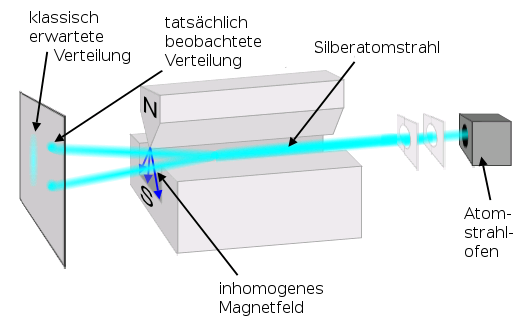
\includegraphics[width=\textwidth]{sterngerlach}}
\caption{\label{fig:SG}Der Stern-Gerlach-Versuch (1922). \href{http://commons.wikimedia.org/wiki/File:Stern-Gerlach_Experiment_de.png?uselang=de}{Grafik: Theresa Knott, Wikimedia Commons}, \href{http://creativecommons.org/licenses/by-sa/3.0/deed.de}{lizenziert unter CreativeCommons-Lizenz by-sa-3.0}.}
\end{figure}

Im in \figurename~\ref{fig:SG} gezeigten und 1922 in Frankfurt a.M.\ durchgef\"uhrten Experiment von Otto Stern und Walther Gerlach werden ungeladene Silberatome in einem Ofen erhitzt. Der aus dem Ofen austretende Strahl ungeladener Silberatome durchl\"auft ein inhomogenes Magnetfeld und trifft auf einen Schirm, auf dem die Intensit\"atsverteilung gemessen wird. Mit der Intensit\"atsverteilung messen wir die Ablenkung der Silberatome im Magnetfeld.

\begin{frage}
 Welche Kraft wirkt auf ein ungeladenes Silberatom in einem inhomogenen Magnetfeld?
\end{frage}
\begin{antw}
Da sie ungeladen sind, wirkt keine Lorentzkraft. Jedes Atom besitzt allerdings ein $5s$-Elektron mit einem Eigendrehimpuls, dem Spin \spin\ mit dem Betrag \hbarh. (Die Drehimpulse der anderen 46 Elektronen heben sich gegenseitig auf.) Daher weist das \emph{Leuchtelektron} und somit das gesamte Atom ein magnetisches Moment \magnmom\ parallel und proportional zum Spin auf: $\magnmom \propto \spin$. Der Betrag des magnetischen Moments des Elektrons (und damit hier des gesamten Atoms) ist das Bohrsche Magneton $\bohrmag = \frac{e}{2m_e}\hbar = |\magnmom|$.
\end{antw}

\begin{frage}
 Wie sieht die Formel der Kraft aus, die auf ein magnetisches Moment \magnmom\ in einem Magnetfeld \magnf\ wirkt?
\end{frage}
\begin{antw}
 Auf ein magnetisches Moment \magnmom\  im (inhomogenen) Magnetfeld \magnf\ wirkt eine Kraft $\mathbf{F} = \nabla (\magnmom \cdot \magnf)$. Wir nehmen an, dass sich das Magnetfeld nur in $z$-Richtung \"andert, sodass $\mathbf{F} = (0,0,F)$ auch nur eine Komponente in $z$-Richtung hat, mit dem Betrag $F= \magnmomm \frac{\partial \magnfm}{\partial z} \cos \alpha$. Hier ist $\alpha = \sphericalangle(\magnmom, \magnf)$ der (konstante) Winkel zwischen magnetischem Moment und Magnetfeld.
\end{antw}

\begin{frage}
 Was misst der Stern-Gerlach-Apparat effektiv?
\end{frage}
\begin{antw}
 Der Stern-Gerlach-Aufbau misst effektiv die Verteilung der Ausrichtungen $\alpha = \sphericalangle(\magnmom, \magnf)$ der magnetischen Momente der Silberatome zum magnetischen Feld. Genauer gesagt misst der Stern-Gerlach-Aufbau die $z$-Komponente $\magnmomm_z$ des magnetischen Moments jedes Silberatoms, und damit die $z$-Komponente $\spinm_z$ des Spins des Leuchtelektrons.
\end{antw}


Die magnetischen Momente \magnmom\ der Silberatome aus dem Ofen sind vor Eintritt in das Magnetfeld zuf\"allig in alle Richtungen orientiert.

\begin{frage}
 Welche qualitative Intensit\"atsverteilung erwarten Sie daher auf dem Schirm?
\end{frage}
\begin{antw}
 Klassisch erwarten wir eine \emph{kontinuierliche} Verteilung zwischen den maximalen Auslenkungen, die gerade der vollst\"andigen Ausrichtung des magnetischen Moments entlang der $z$-Richtung entsprechen ($\magnmomm_z = \pm |\magnmom|$). Wegen der zuf\"alligen Orientierung der magnetischen Momente kommen auch dazwischen alle Werte vor.
\end{antw}

\begin{erg}
 Tats\"achlich beobachten wir im Stern-Gerlach-Experiment, dass der Strahl im Apparat aufgespalten wird und wir zwei \emph{diskrete} Komponenten $z_+$ und $z_-$ erhalten, die gerade den vollst\"andigen Ausrichtungen der magnetischen Momente entsprechen!

Nach der Messung erhalten wir also zwei getrennte Teilstrahlen mit nur den beiden diskreten Werten $\spinm_z = +\hbarh$ and $\spinm_z = -\hbarh$ f\"ur den Spin.
\end{erg}


\begin{zfrage}
 Warum richten sich nicht schon klassisch gesehen alle magnetischen Momente im Magnetfeld aus? 
\end{zfrage}
\begin{antw}
 Magnetische Momente von ruhenden K\"orpern (Stabmagnete z.B.) richten sich in der Tat am Magnetfeld aus. Elektronenspins stehen aber f\"ur eine Eigen\emph{rotation}, und magnetische Momente \magnmom\ rotierender K\"orper behalten ihren Winkel zur Feldrichtung \magnf: sie richten sich nicht aus, sondern pr\"azessieren (wie ein mechanischer Kreisel) unter dem Drehmoment $\magnmom \times \magnf$ um die durch die Feldrichtung \magnf\ gegebene Achse. Dabei bleibt der Winkel zu dieser Achse konstant. W\"urden sich die Elektronenspins tats\"achlich im Magnetfeld ausrichten, m\"ussten zudem alle in Richtung des Magnetfeldes zeigen, und keiner in entgegengesetzte Richtung (wie es aber beim Stern-Gerlach-Experiment beobachtet wird).
\end{antw}

\subsection{Hintereinanderschaltung von Stern-Gerlach-Apparaturen}
\begin{frage}
 Was erwarten Sie (klassisch): Welche Teilstrahlen treten auf, wenn der $z_-$-Teilstrahl aus einem Stern-Gerlach-Apparat $\sg_z$ blockiert wird und nur der $z_+$-Teilstrahl in einen weiteren Stern-Gerlach-Apparat $\sg_z$ geschickt wird?
\end{frage}
\begin{obs}
 Siehe \figurename{}~\ref{fig:seqSQ} oben: Es \"andert sich nichts. Die Spins bleiben in $z_+$-Richtung ausgerichtet.
\end{obs}

\begin{frage}
 Der $z_+$-Teilstrahl aus einer Stern-Gerlach-Apparatur $\sg_z$ wird in einer in $x$-Richtung angeordneten Stern-Gerlach-Apparatur $\sg_x$ wieder zur H\"alfte in zwei Komponenten $x_+$ und $x_-$ aufgeteilt, siehe \figurename{}~\ref{fig:seqSQ} Mitte. Wie erkl\"aren Sie sich dieses Ergebnis?
\end{frage}
Man k\"onnte klassisch vermuten, dass die Spins der Leuchtelektronen der Silberatome im $z_+$-Strahl je zur H\"alfte durch $\spinm_z = +\hbarh, \spinm_x = +\hbarh$ und $\spinm_z = +\hbarh, \spinm_x = -\hbarh$ bestimmt sind.

Aber:
\begin{obs}
Schickt man nur den $x_+$-Teilstrahl aus einer Stern-Gerlach-Apparatur $\sg_x$, der nur aus dem $z_+$-Teilstrahl einer $\sg_z$-Apparatur gewonnen wurde, erneut durch eine $\sg_z$-Apparatur, so spaltet sich dieser erneut je zur H\"alfte in $z_+$ und $z_-$ auf!
\end{obs}

Willkommen in der Quantenmechanik! Denn:
\begin{erg}
 Die Messung von $\spinm_x$ durch die $\sg_x$-Apparatur verbunden mit der Selektion des $x_+$-Zustands vernichtet alle vorherige Information \"uber den Zustand $z_+$. $\spinm_z$ und $\spinm_x$ lassen sich nicht gleichzeitig bestimmen!
\end{erg}

\begin{figure}
 \href{http://commons.wikimedia.org/wiki/File:Sg-seq.svg}{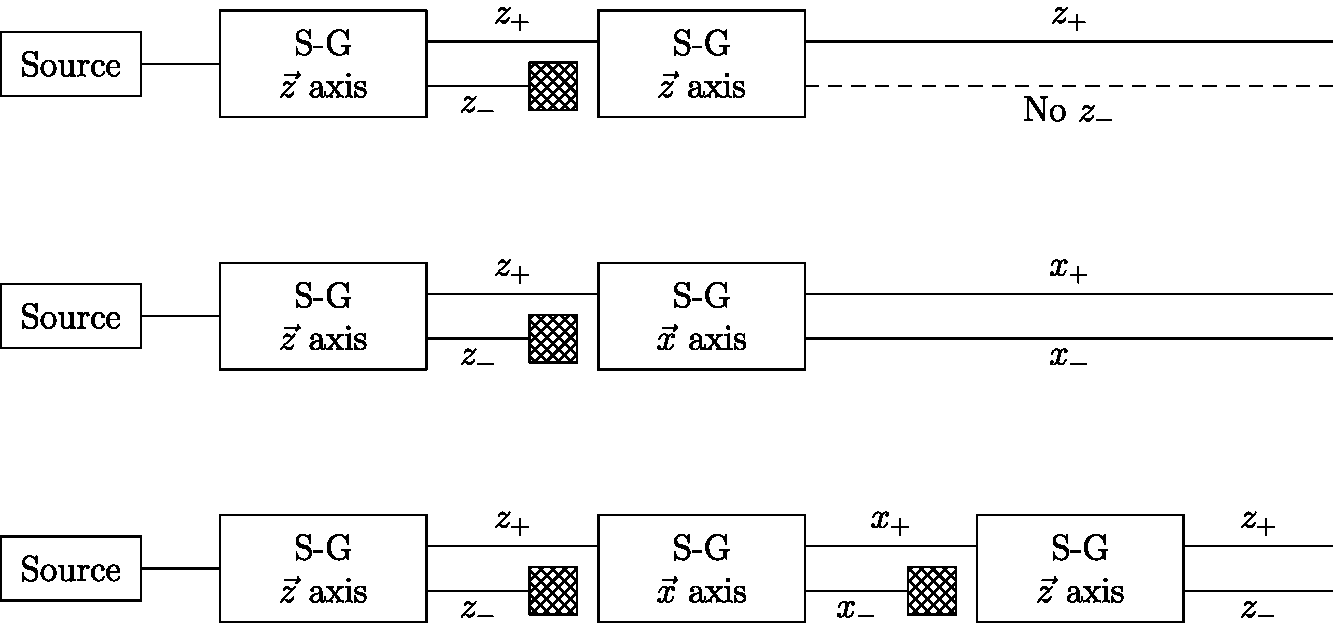
\includegraphics[width=\textwidth]{sequentieller-sterngerlach}}
\caption{\label{fig:seqSQ}Sequentielle Stern-Gerlach-Versuche. \href{http://commons.wikimedia.org/wiki/File:Sg-seq.svg}{Grafik: Francesco Versaci, Wikimedia Commons}, Public Domain.}
\end{figure}


\section{Zust\"ande, Observable, Operatoren}

\subsection{Der quantenmechanische Zustand (ket-Vektoren)}

Der sequentielle Stern-Gerlach-Versuch widerlegt unsere klassische Intuition: physikalische Messungen ver\"andern n\"amlich im Allgemeinen den Zustand unseres Systems! Ein weiterer Widerspruch zu unserer klassischen Intuition ist, dass wir nicht alle physikalischen Gr\"o\ss{}en gleichzeitig messen k\"onnen. Wir k\"onnen daher nicht alles gleichzeitig \"uber einen Zustand wissen.

Wir definieren daher nach \textcite{Nolting}:

\begin{post}
 Gleichzeitige Messung eines maximalen Satzes von \enquote{vertr\"aglichen}, d.h. simultan messbaren, Eigenschaften \enquote{pr\"apariert} einen \enquote{reinen} quantenmechanischen Zustand.
\end{post}

\begin{bsp}
 Bez\"uglich des Elektronenspins haben wir bereits (reine) Zust\"ande kennengelernt: \szus\ und \szds.
\end{bsp}

Wie k\"onnen wir nun mit diesen abstrakten quantenmechanischen Zust\"anden rechnen, also konkrete physikalische Vorhersagen treffen?

\begin{post}
 In der Quantenmechanik wird ein physikalisches System durch einen \emph{Zustandsvektor} \keta\ in einem komplexen Vektorraum, einem sogenannten Hilbertraum \hs, repr\"asentiert. \keta\ enth\"alt die gesamte Information \"uber den physikalischen Zustand. 
\end{post}

Nach Dirac nennen wir einen Zustandsvektor \keta\ auch \emph{ket-Vektor} (kurz: \emph{ket}), und den Hilbertraum \emph{ket-Raum}.

Wie Vektoren k\"onnen wir Kets $\keta, \ketb \in \hs$ addieren, die Summe ist wieder ein Ket:
\begin{equation*}
 \keta + \ketb = \ket{\gamma} \in \hs
\end{equation*}
Wie ein Vektor l\"asst sich auch ein Ket mit einer komplexen Zahl $c \in \comps$ multiplizieren, und wir erhalten wieder ein Ket:
\begin{equation*}
 c \keta = \keta c \in \hs
\end{equation*}

\begin{post}
 $\keta$ und $c \keta$ mit $c \neq 0$ sind zwar zwei verschiedene Elemente im Ket-Raum \hs, repr\"asentieren aber den selben physikalischen Zustand.
\end{post}

\subsection{Observablen}
Wie k\"onnen wir nun konkret etwas \"uber unser physikalisches System erfahren, das durch einen abstrakten Zustandsvektor repr\"asentiert wird? Durch messbare physikalische Gr\"o\ss{}en:

\begin{post}
 Messbare physikalische Gr\"o\ss{}en (\emph{Observablen}) werden durch lineare Abbildungen (\emph{Operatoren}) auf dem Ket-Raum repr\"asentiert.
\end{post}
Eine Observable $A$ wird also repr\"asentiert durch den Operator $\op{A}: \hs \rightarrow \hs$, $\op{A}( \keta) \equiv \op{A}\keta \equiv A \keta \in \hs$ ist wieder ein Ket.
\begin{konv}
 Mit der Schreibweise $A$ ist oft der Operator $\op{A}$ der Observablen $A$ gemeint!
\end{konv}
Im Allgemeinen ist das Ket $\op{A} \keta$ nicht gleich einer komplexen Zahl multipliziert mit $\keta$! Aber:
\begin{defn}
Die Eigenvektoren $\ket{a_i}$ der linearen Abbildung $\op{A}$ bezeichnen wir auch als \emph{Eigenkets} oder \emph{Eigenzust\"ande} des physikalischen Systems bez\"uglich der Observablen $A$, mit den jeweiligen Eigenwerten $a_i \in \comps$:
\begin{equation*}
 \op{A} \ket{a_i} = a_i \ket{a_i}
\end{equation*}
\end{defn}

\begin{bsp}
 Spin-$\frac{1}{2}$-Systeme haben bez\"uglich der $z$-Richtung die Eigenvektoren \szus\ und \szds\ mit den Eigenwerten $+\hbarh$ und $-\hbarh$:
 \begin{align*}
  \szop \szus &= + \hbarh \szus \\
  \szop \szds &= - \hbarh \szds \\
  \text{oder auch:} \quad \szop \szs &= \pm \hbarh \szs
 \end{align*}

\end{bsp}

\subsection{Duale Zustandsvektoren (bras)}
\begin{post}
 Zu jedem Zustandsvektor $\keta \in \hs$ existiert ein \emph{duales} Ket $\braa \in \ds{\hs}$ im Dualraum von \hs, dem Raum \ds{\hs}\ der linearen Abbildungen $\hs \rightarrow \comps$. Wir bezeichnen $\braa$ auch als das zum Ket $\keta$ korrespondierende \emph{bra} (oder den \emph{bra-Vektor}), und \ds{\hs}\ als \emph{bra-Raum}, und schreiben:
\begin{equation}
 \keta \dc \braa
\end{equation}
 Wir postulieren weiterhin, dass wir mit den korrespondierenden Bras wie mit den Kets rechnen k\"onnen:
\begin{equation}
 c_{\alpha} \keta + c_{\beta} \ketb \dc \cc{c_{\alpha}} \braa + \cc{c_{\beta}} ,
\end{equation}
wobei die Vorfaktoren durch duale Korrespondenz komplex konjugiert werden!
\end{post}

\subsection{Inneres Produkt (Skalarprodukt)}
\begin{post}
 Um die Dirac'sche Bra-ket-Notation zu vollenden, postulieren wir nun noch das \emph{innere Produkt} (Skalarprodukt) $\braket{\beta | \alpha} \in \comps$ eines Bras $\brab$ und eines Kets $\keta$:
\begin{equation}
 \braket{\beta | \alpha} \equiv \brab \cdot \keta \equiv \brab ( \keta ) \in \comps
\end{equation}
Das innere Produkt habe folgende Eigenschaften:
\begin{align}
 \braket{\beta | \alpha} &= \cc{\braket{\alpha | \beta}} \\
\braket{\alpha | \alpha} &\geq 0 \qquad \text{\enquote{positiv definit}} 
\end{align}

\end{post}
 
\begin{defn}
 Wir nennen zwei physikalische Zust\"ande bzw. ihre repr\"asentierenden Zustandsvektoren \keta, \ketb, \emph{orthogonal}, wenn gilt $\braket{\beta | \alpha} = 0$.
\end{defn}
\begin{notiz}
 \begin{equation}
  \braket{\beta | \alpha} = 0 \Leftrightarrow \braket{\alpha | \beta} = 0
 \end{equation}
\end{notiz}

\begin{defn}
 Wir nennen einen Zustandsvektor \keta\ \emph{normiert}, wenn $\braket{\alpha | \alpha} = 1$ gilt.
\end{defn}
\begin{konv}
 Da ein physikalischer Zustand von einem Ket nur bis auf einen komplexen Vorfaktor festgelegt ist, k\"onnen wir festlegen, dass wir im folgenden nur noch normierte Zustandsvektoren betrachten.
\end{konv}

\subsection{Operatoren}
Wenden wir uns nun wieder den Operatoren zu, und zwar ganz allgemein linearen Abbildungen auf dem Ketraum \hs, nicht nur solchen, die physikalisch messbaren Gr\"o\ss{}en (Observablen) entsprechen.

\begin{eig}
Auf ein Ket \keta\ wirkt ein Operator \opx\ ganz normal \enquote{von links}, d.h. $\opx(\keta) \equiv \opx \keta \in \hs$ ist wieder ein Ket.
\end{eig}

\begin{eig}
 Wie Funktionen auf den reellen Zahlen auch werden Operatoren dar\"uber definiert, wie sie auf (alle) Kets wirken.
\end{eig}

\begin{bsp}
 Zwei Operatoren $\opx, \opy$ sind gleich, $\opx=\opy$, wenn $\opx \keta = \opy \keta$ f\"ur alle Kets $\keta$ gilt.
\end{bsp}

\begin{eig}
Operatoren lassen sich \enquote{wie Zahlen} zu neuen Operatoren addieren, kommutativ und assoziativ:
\begin{align}
\opx + \opy &= \opy + \opx \\
\opx + (\opy + \op{Z}) &= (\opx + \opy) + \op{Z}
\end{align}
\end{eig}

\begin{eig}
 Operatoren sind linear:
 \begin{equation}
  \opx(\ca \keta + \cb \ketb) = \ca \opx \keta + \cb \opx \ketb
 \end{equation}
\end{eig}

\begin{post}
Operatoren wirken auch auf Bras, und zwar \emph{von rechts}!
\begin{equation}
\opx(\braa) \equiv \braa \opx \in \ds
\end{equation} 
$\braa\opx$ ist wieder ein Bra! Ein Operator \opx\ wirke gerade so auf einen Bra-Vektor \braa, dass f\"ur beliebe \ketb\ gilt:
 \begin{equation}
  (\braa \opx) \cdot \ketb = (\braa) \cdot (\opx \ketb) \in \comps
 \end{equation}
 Dies ist eine komplexe Zahl, da es sich um ein Skalarprodukt aus dem Bra $\braa\opx$ und dem Ket \ketb\ bzw. aus dem Bra $\braa$ und dem Ket $\opx\ketb$ handelt.
\end{post}
\begin{konv}
 Da hier wieder ein Assoziativgesetz gilt, k\"onnen wir die Klammern auch weglassen und schreiben:
 \begin{equation}
  (\braa \opx) \cdot \ketb = (\braa) \cdot (\opx \ketb) \equiv \braa \opx \ketb
 \end{equation}
\end{konv}

\begin{eig}
 Wir k\"onnen Operatoren multiplizieren, d.h. hintereinander auf einen Zustandsvektor \keta\ anwenden, und wieder ein Ket erhalten: $\opy \opx \keta \equiv \opy ( \opx \keta) \in \hs$.
\end{eig}

\begin{eig}
 Die Reihenfolge ist bei der Multiplikation (Hintereinanderausf\"uhrung) von Operatoren im Allgemeinen nicht egal! Im Allgemeinen \emph{kommutieren} Operatoren \emph{nicht}:
 \begin{equation}
  \opx \opy \neq \opy \opx
 \end{equation}
\end{eig}
\begin{eig}
 Die Multiplikation von Operatoren ist aber assoziativ, d.h.
 \begin{gather}
  \opx (\opy \op{Z}) = (\opx \opy) \op{Z} \equiv \opx \opy \op{Z} \\
  \opx(\opy \keta) = (\opx \opy) \keta \equiv \opx \opy \keta \\
  (\brab \opx) \opy = \brab (\opx \opy)\equiv \brab \opx \opy
 \end{gather}

\end{eig}

\subsection{Der hermitesch adjungierte Operator}
\begin{notiz}
 Im Allgemeinen korrespondiert das Bra $\braa \opx$ nicht mit dem Ket $\opx \keta$! Daher:
\end{notiz}

\begin{defn}
 Sei \opx\ ein Operator. Der zu \opx\ \emph{hermitesch adjungierte Operator} oder auch einfach \emph{adjungierte Operator} \opxh\ sei f\"ur alle Kets \keta\ definiert \"uber die duale Korrespondenz
 \begin{equation}
  \opx \keta \dc \braa \opxh
 \end{equation}

\end{defn}

\begin{defn}
 Gilt f\"ur einen Operator $\opxh = \opx$, d.h. $\opx \keta \dc \braa \opx$ f\"ur alle Kets \keta, so hei\ss{}t \opx\ \emph{hermitesch}.
\end{defn}

\begin{eig}
 \begin{equation}
  \herm{(\opx \opy)} = \opyh \opxh
 \end{equation}

\end{eig}
\begin{aufg}
 Zeigen Sie $\herm{(\opx \opy)} = \opyh \opxh$!
\end{aufg}
\begin{tipp}
\begin{enumerate}
 \item Auf beiden Seiten der Gleichung steht ein Operator. Wann sind diese beiden Operatoren gleich?
 \item Assoziativgesetz und Definition der hermitesch Adjungierten jeweils einmal f\"ur \opx\ und \opy\ getrennt anwenden.
\end{enumerate}
\end{tipp}
\begin{loes}
 Die Operatoren sind gleich, wenn sie f\"ur alle Zustandsvektoren \keta\ das gleiche Ergebnis liefern. Sei \keta\ daher nun ein beliebiges Ket.
 \begin{align}
  \opx \opy \keta &= \opx ( \opy \keta) \tag{Assoziativgesetz}\\
  &\dc \Bra{\opy \keta} \opxh \tag{Definition von \opxh}\\
  &= (\braa \opyh) \opxh \tag{$\Bra{\opy \keta} = \braa \opyh$, Definition von \opyh} \\
  &= \braa \opyh \opxh \tag{Assoziativgesetz}
 \end{align}

 \qedsymbol
\end{loes}

\begin{aufg} \label{aufg:ccadjmatrixelement}
 Zeigen Sie $\brab\opx\keta = \cc{\braa\opxh\ketb}$.
\end{aufg}
\begin{loes}
 \begin{align}
  \brab\opx\keta &= \brab \cdot \left(\opx\keta\right) \tag{Assoziativgesetz} \\
  &= \cc{\left(\left(\braa\opxh\right) \cdot \ketb \right)} \tag{Eigenschaft des Skalarprodukts} \\
  &= \cc{\Braket{\alpha | \opxh | \beta}} \tag{Assoziativgesetz}
 \end{align}
 \qedsymbol
\end{loes}

\begin{notiz}
 F\"ur hermitesche Operatoren $\opxh = \opx$ gilt demnach:
 \begin{equation}
  \Braket{\beta | \opx | \alpha} = \cc{\Braket{\alpha | \opx | \beta}}
 \end{equation}

\end{notiz}


\subsection{Das \"au\ss{}ere Produkt}
\begin{post}
 Sei \ketb\ ein Ket-Vektor und \braa\ ein Bra-Vektor. Wir postulieren nun ein \emph{\"au\ss{}eres Produkt} als einen Operator $\opx = \ketb\braa$, der wie folgt auf ein beliebiges Ket $\ket{\gamma}$ bzw. Bra $\bra{\gamma}$ wirkt:
 \begin{align}
  \opx (\ket{\gamma}) &= (\ketb\braa)(\ket{\gamma}) \equiv \ketb (\braket{\alpha|\gamma}) \\
  \bra{\gamma} \opx &= \bra{\gamma} (\ketb\braa) \equiv (\braket{\gamma | \beta}) \braa
 \end{align}
 $\braket{\alpha|\gamma}$ ist wieder das Skalarprodukt, eine komplexe Zahl, die mit dem Ket \ketb\ multipliziert wird, sodass am Ende wieder ein Ket herauskommt.
\end{post}
\begin{notiz}
 Der Operator $\ketb\braa$ projiziert ein Ket $\ket{\gamma}$ auf die Richtung des Ket-Vektors \ketb! Dabei gibt der Vorfaktor $\braket{\alpha|\gamma}$ gerade an, wie sehr $\ket{\gamma}$ mit dem Zustand \keta\ \"uberlappt!
\end{notiz}
\begin{konv}
 Wenn die Notation eindeutig bleibt, schreiben wir auch einfach:
 \begin{equation}
  (\ketb\braa)(\ket{\gamma}) \equiv \ketb (\braket{\alpha|\gamma}) \equiv \ketb\braket{\alpha|\gamma}
 \end{equation}
 Dies verdeutlicht das f\"ur das \"au\ss{}ere Produkt geltende Assoziativgesetz!
\end{konv}

\begin{aufg}
 Zeigen Sie $\herm{(\ketb\braa)} = \keta\brab$.
\end{aufg}
\begin{tipp}
 \begin{enumerate}
  \item Wann sind zwei Operatoren gleich? Wenn sie auf ein beliebiges Ket angewendet das selbe Ergebnis liefern.
  \item F\"uhren Sie die duale Korrespondenz des Operators $(\ketb\braa)$ auf die bekannte duale Korrespondenz des resultierenden Ket-Vektors \ketb\ zur\"uck.
 \end{enumerate}
\end{tipp}
\begin{loes}
 Sei $\ket{\gamma}$ ein beliebiger Zustandsvektor.
 \begin{align}
 (\ketb\braa) \ket{\gamma} &= \ketb (\braket{\alpha | \gamma}) \tag{Definition des \"au\ss{}eren Produkts} \\
 &\dc \cc{(\braket{\alpha | \gamma})} \brab \tag{Duale Korrespondenz von \ketb} \\
 &= (\braket{\gamma | \alpha}) \brab \tag{Eigenschaft des Skalarprodukts} \\
 &= \bra{\gamma} (\keta\brab) \tag{Definition des \"au\ss{}eren Produkts} \\
 \Leftrightarrow  (\ketb\braa) \ket{\gamma} &\dc \bra{\gamma} (\keta\brab)
 \end{align}
\qedsymbol
\end{loes}

\subsection{Hermitesche Operatoren}
Nun betrachten wir die Eigenwerte und Eigenzust\"ande hermitescher Operatoren \opa\ ($\herm{\opa} = \opa$).
\begin{eig}
 Die Eigenwerte $a_i$ eines hermiteschen Operators \opa\ mit $\opa \ket{a_i} = a_i \ket{a_i}$ sind reell. Die Eigenzust\"ande von \opa\ zu verschiedenen Eigenwerten sind orthogonal: $\braket{a_j|a_i} = 0$ f\"ur $a_j \neq a_i$.
\end{eig}
\begin{aufg}
 Zeigen Sie diese beiden Eigenschaften eines hermiteschen Operators \opa.
\end{aufg}
\begin{tipp}
 Was sind die Eigenwerte und Eigenvektoren von \opa\ im Bra-Raum? Geben Sie hierzu die Eigenwertgleichung im Bra-Raum an, die mit der Eigenwertgleichung $\opa \ket{a_i} = a_i \ket{a_i} $ dual korrespondiert.
\end{tipp}
\begin{loes}
 Die Eigenvektoren von \opa\ im Bra-Raum sind gerade die mit den Eigenvektoren dual korrespondierenden Bras $\bra{a_i}$, mit den komplex konjugierten Eigenwerten $\cc{a_i}$. F\"ur beliebige Eigenzust\"ande $\ket{a_i}, \ket{a_j}$ gilt:
 \begin{align}
 \opa \ket{a_i} &= a_i\ket{a_i} \tag{Eigenwertgleichung f\"ur \opa\ im Ketraum} \\
 \Rightarrow \braket{a_j | \opa | a_i} &= \braket{a_j | a_i | a_i} = a_i \braket{a_j|a_i} \\
 \bra{a_j} \opa &= \cc{a_j} \bra{a_j} \tag{Eigenwertgleichung im Braraum} \\
 \Rightarrow \braket{a_j | \opa | a_i} &= \cc{a_j} \braket{a_j|a_i} \\
 \Rightarrow a_i \braket{a_j | a_i} &= \cc{a_j} \braket{a_j | a_i} \\
 \Rightarrow (a_i - \cc{a_j}) \braket{a_j | a_i} &= 0
 \end{align}
 F\"ur den Fall $\ket{a_j} = \ket{a_i}$ ist $\braket{a_j | a_i} = \braket{a_i | a_i} = 1 \neq 0$, also muss $a_i = \cc{a_j} = \cc{a_i}$ sein und damit $a_i \in \reals$. F\"ur den Fall $a_j \neq a_i$ muss gelten $\braket{a_j | a_i} = 0$. \qedsymbol
\end{loes}

\subsection{Die orthonormale Basis von Eigenzust\"anden einer Observablen}
\begin{post}
 Gegeben sei eine Observable $A$ mit den Eigenzust\"anden $\ket{a_i}$. Wir k\"onnen jeden Zustandsvektor $\keta$ nach diesen Eigenzust\"anden entwickeln, sprich als Summe der Eigenzust\"ande mit komplexen Vorfaktoren $c_i \in \comps$ schreiben:
\begin{equation}
 \keta = \sum_i c_i \ket{a_i}
\end{equation}
Wir sagen auch: Die Eigenzust\"ande $\ket{a_i}$ spannen den Ketraum $\hs$ auf. Die komplexen \emph{Entwicklungskoeffizienten} $c_i$ von \keta\ sind gerade gegeben durch
 \begin{equation}
  c_i = \braket{a_i | \alpha} \in \comps
 \end{equation}
Entsprechend gelte mit
\begin{equation}
 \keta = \sum_i \ket{a_i}\braket{a_i|\alpha},
\end{equation}
da \keta\ ein beliebiger Zustandsvektor ist:
\begin{equation}
 \sum_i\ket{a_i}\bra{a_i} = \opi
\end{equation}
\opi\ ist der Identit\"atsoperator, der also alle Kets $\keta$ auf sich selbst abbildet: $\opi \keta = \keta$.
\end{post}

\begin{defn}
 Die Einzel-Operatoren $\ket{a_i}\bra{a_i}$ der Zerlegung von \opi\ nennen wir \emph{Projektionsoperator} zum Eigenzustand $\ket{a_i}$, da sie einen beliebigen Zustand \keta\ auf die Richtung von $\ket{a_i}$ projizieren, mit dem \enquote{\"Uberlapp} (Vorfaktor) $c_i = \braket{a_i | \alpha}$.
\end{defn}

\begin{defn}
 Wir w\"ahlen die Eigenzust\"ande $\ket{a_i}$ einer Observablen $A$ so, dass sie ein \emph{vollst\"andiges Orthonormalsystem} (\emph{VONS}) $\{\ket{a_i}\}_i$ bilden:
 \begin{equation}
  \braket{a_j | a_i} = \delta_{ij}
 \end{equation}
\end{defn}

\begin{aufg}
 Zeigen Sie, dass die Summe der Betragsquadrate der Entwicklungskoeffizienten $c_i$ von einem beliebigen Zustand \keta\ bez\"uglich des VONS $\{\ket{a_i}\}_i$ gerade $1$ ergibt:
 \begin{equation}
  \sum_i |c_i|^2 = 1
 \end{equation}
\end{aufg}
\begin{tipp}
 Geschicktes Identifizieren der \opi!
\end{tipp}
\begin{loes}
 \begin{align}
  \sum_i |c_i|^2 &= \sum_i \lvert\braket{a_i|\alpha}\rvert^2 \\
  &= \sum_i \cc{\braket{a_i | \alpha}} \braket{a_i|\alpha} \\
  &= \sum_i \braket{\alpha | a_i} \braket{a_i|\alpha} \\
  &= \braa \left(\sum_i \ket{a_i}\bra{a_i} \right) \keta \\
  &= \braa \opi \keta = \braket{\alpha | \alpha} = 1.
 \end{align}
 \qedsymbol
\end{loes}


\subsection{Matrixdarstellung von Operatoren}
\emph{Wir erinnern uns daran, dass unsere Operatoren lineare Abbildungen auf einem Vektorraum sind, und wir zudem zu einer Observablen $A$ eine Basis (VONS) $\{\ket{a_i}\}_i$ von Eigenzust\"anden dieser Observablen zur Verf\"ugung haben. Damit k\"onnen wir Operatoren auch in gewohnter Form als Matrizen bez\"uglich dieser Basis darstellen!}
\begin{defn}
 Gegeben eine Basis von Eigenzust\"anden (VONS)  $\{\ket{a_i}\}_i$ einer Observablen $A$, k\"onnen wir einen Operator \opx\ durch Hinzuf\"ugen von \opi-en schreiben als:
 \begin{align}
  \opx &= \opi \cdot  \opx \cdot \opi = \left(\opix{i}{a_i} \right) \opx \left(\opix{j}{a_j}\right) \\
  &= \sum_{i,j} \ket{a_i} \Braket{a_i | \opx | a_j} \bra{a_j} \\
  &\equiv \sum_{i,j} X_{ij} \ket{a_i}\bra{a_j}
 \end{align}
 $X_{ij} = \Braket{a_i | \opx | a_j} \in \comps$ hei\ss{}t das \emph{Matrixelement $(i,j)$} von \opx\ bez\"uglich der Basis $\{\ket{a_i}\}_i$.
\end{defn}
\begin{notiz}
 Wir haben den Operator \opx\ also zerlegt in eine Summe von Operatoren $\ket{a_i}\bra{a_j}$ mit den Matrixelementen $X_{ij} = \braket{a_i | \opx | a_j}$ als komplexen Koeffizienten.
\end{notiz}
\begin{aufg}
 Seien die Matrixelemente $X_{ij} = \braket{a_i | \opx | a_j}$ eines Operators \opx\ bez\"uglich eines VONS $\{\ket{a_i}\}_i$ gegeben. Geben Sie das Matrixelement $\braket{a_i | \opxh | a_j}$ des adjungierten Operators \opxh\ an!
\end{aufg}
\begin{tipp}
 Wir haben das schon berechnet!
\end{tipp}
\begin{loes}
 \begin{equation}
  \braket{a_i | \opxh | a_j} = \cc{\braket{a_j | \opx | a_i}}
 \end{equation}
 Siehe Aufgabe \ref{aufg:ccadjmatrixelement}! \qedsymbol
\end{loes}


\begin{defn}
 Wir nennen die Matrix
 \begin{equation}
  \opx \doteq \begin{pmatrix}
            \braket{a_1 | \opx | a_1} & \braket{a_1 | \opx | a_2} & \cdots \\
            \braket{a_2 | \opx | a_1} & \braket{a_2 | \opx | a_2} & \cdots \\
            \vdots & \vdots & \ddots
           \end{pmatrix}
 \end{equation}
 die \emph{Matrixdarstellung} des Operators \opx\ bez\"uglich des VONS $\{\ket{a_i}\}_i$. Der Eintrag in der $i$-ten Zeile und $j$-ten Spalte ist gerade das Matrixelement $X_{ij} = \braket{a_i | \opx | a_j}$.
\end{defn}
\begin{notiz}
 Die Matrixdarstellung eines Operators h\"angt somit von der gew\"ahlten Basis ab! Daher ist der Operator nicht \emph{gleich} der Matrix, und wir w\"ahlen das Symbol \enquote{$\doteq$}. Oft schreibt man aber auch \enquote{$=$}, insbesondere wenn man in einer festen Basis von Eigenzust\"anden rechnet.
\end{notiz}
\begin{eig}
 Die Matrixdarstellung eines Operators ist quadratisch und hat so viele Zeilen bzw. Spalten, wie es Basiszust\"ande gibt. Die Zahl der Basiszust\"ande entspricht der Dimension unseres Zustandsraums (Hilbertraums) \hs.
\end{eig}
\begin{aufg}
 Sei die Matrixdarstellung eines Operators \opx\ bez\"uglich einer Basis $\{\ket{a_i}\}_i$ gegeben. Wie erhalten Sie hieraus die Matrixdarstellung von \opxh?
\end{aufg}
\begin{loes}
 Mit $\braket{a_i | \opxh | a_j} = \cc{\braket{a_j | \opx | a_i}}$ wissen wir, dass das Matrixelement von \opxh\ in der $i$-ten Zeile und $j$-ten Spalte gerade das komplex konjugierte Matrixelement von \opx\ in der $j$-ten Zeile und $i$-ten Spalte ist. Die Matrixdarstellung von \opxh\ ist also die transponierte und komplex konjugierte Matrixdarstellung von \opx.
\end{loes}


\section{Physikalische Interpretation}

\section{Das Spin-$\frac{1}{2}$-System und die Pauli-Matrizen}

\section{Die Wellenfunktion im Dirac-Formalismus}

\section{Die Dynamik von Quantensystemen}
\subsection{Zeitentwicklung der Zust\"ande (Schr\"odinger-Bild)}

\subsection{Zeitentwicklung der Observablen (Heisenberg-Bild)}